% Template for Cogsci submission with R Markdown

% Stuff changed from original Markdown PLOS Template
\documentclass[10pt, letterpaper]{article}

\usepackage{cogsci}
\usepackage{pslatex}
\usepackage{float}
\usepackage{caption}

% amsmath package, useful for mathematical formulas
\usepackage{amsmath}

% amssymb package, useful for mathematical symbols
\usepackage{amssymb}

% hyperref package, useful for hyperlinks
\usepackage{hyperref}

% graphicx package, useful for including eps and pdf graphics
% include graphics with the command \includegraphics
\usepackage{graphicx}

% Sweave(-like)
\usepackage{fancyvrb}
\DefineVerbatimEnvironment{Sinput}{Verbatim}{fontshape=sl}
\DefineVerbatimEnvironment{Soutput}{Verbatim}{}
\DefineVerbatimEnvironment{Scode}{Verbatim}{fontshape=sl}
\newenvironment{Schunk}{}{}
\DefineVerbatimEnvironment{Code}{Verbatim}{}
\DefineVerbatimEnvironment{CodeInput}{Verbatim}{fontshape=sl}
\DefineVerbatimEnvironment{CodeOutput}{Verbatim}{}
\newenvironment{CodeChunk}{}{}

% cite package, to clean up citations in the main text. Do not remove.
\usepackage{cite}

\usepackage{color}

% Use doublespacing - comment out for single spacing
%\usepackage{setspace}
%\doublespacing


% % Text layout
% \topmargin 0.0cm
% \oddsidemargin 0.5cm
% \evensidemargin 0.5cm
% \textwidth 16cm
% \textheight 21cm

\title{Seeking visual information to support spoken language comprehension in
noisy environments}


\author{ {\large \bf Kyle MacDonald}$^1$ (kylem4@stanford.edu), {\large \bf Virginia Marchman}$^1$ (marchman@stanford.edu),  \\ {\large \bf Anne Fernald}$^1$ (afernald@stanford.edu), {\large \bf Michael C. Frank}$^1$ (mcfrank@stanford.edu) 
  \\ $^1$ Department of Psychology Stanford University}

\begin{document}

\maketitle

\begin{abstract}
Language comprehension in grounded contexts is facilitated by
integrating visual information with the incoming linguistic signal. But
the value of visual information varies across different language
processing contexts -- e.g., becoming more useful in noisy auditory
environments. Do listeners take this information into account when
deciding where to fixate?Here, we report two experiments supporting the
hypothesis that listeners adapt gaze patterns to seek higher value
visual information when it is useful for establishing reference. First,
we show that adults (n=33) and children (n=40, 3-5 y.o.) delayed their
eye movements away from a speaker while processing familiar nouns in
noise. Intrestingly, the decision to delay resulted in a speed-accuracy
tradeoff, with more accurate shifts and fewer random responses (E1).
Next, we present results showing the limits of this adaptive response:
adults (n=33) and children (n=54, 3-5 y.o.) did not delay eye movements
to wait for a post-nominal social cue (eye gaze) when the auditory
signal was sufficient to establish reference (E2). Together, these
results suggest that the dynamics of eye movements during language
comprehension flexibly adapt to the processing context, and even very
young listeners will seek higher value visual information when it is
useful for comprehension.

\textbf{Keywords:}
eye movements; language processing; information-seeking; speech in
noise; social cue processing
\end{abstract}

\section{Introduction}\label{introduction}

The study of eye movements during language comprehension has provided
fundamental insights into the interaction between conceptual
representations of the world and the incoming linguistic signal. For
example, research shows that adults and children will rapidly shift
visual attention upon hearing the name of an object in the visual scene,
with a high proportion of shifts occurring prior to the offset of the
word (Allopenna, Magnuson, \& Tanenhaus, 1998; Tanenhaus,
Spivey-Knowlton, Eberhard, \& Sedivy, 1995). Moreover, researchers have
found that conceptual representations activated by fixations to the
visual world can modulate subsequent eye movements during language
processing (Altmann \& Kamide, 2007).

The majority of this work has used eye movements as a measure of the
output of the underlying language comprehension process, often using
linguistic stimuli that come from a disembodied voice. But in real world
contexts, people also gather information about the linguistic signal by
fixating on the language source. Consider a speaker who asks you to
``Pass the salt'' but you are in a noisy room, making it difficult to
understand the request. Here, comprehension can be facilitated by
gathering information via (a) fixations to the nonlinguistic visual
world (i.e., encoding the objects that are present in the scene) or (b)
fixations to the speaker (i.e., reading lips or perhaps the direction of
gaze).

But, this situation creates a tradeoff where the listener must decide
what kind of information to gather and at what time. How do we decide
where to look? We propose that people modulate their eye movements
during language comprehension in response to tradeoffs in the value of
gathering different kinds of information. We test this adaptive tradeoff
account using two case studies that manipulate the value of different
fixation locations for language understanding: a) a comparison of
processing sign vs.~spoken language in children (E1), and b) a
comparison of processing printed text vs.~spoken language in adults
(E2). Our key prediction is that competition for visual attention will
make gaze shifts away from the language source less valuable than
fixating the source of the linguistic signal, leading people to generate
fewer exploratory, nonlanguage-driven eye movements.

\section{Experiment 1}\label{experiment-1}

E1 provides an initial test of our adaptive tradeoffs account. We
compared eye movements of children learning ASL to children learning a
spoken language using parallel real-time language comprehension tasks
where children processed familiar sentences (e.g., ``Where's the
ball?'') while looking at a simplified visual world with 3 fixation
targets (a center stimulus that varied by condition, a target picture,
and a distracter picture; see Fig 1). The spoken language data are a
reanalysis of three unpublished data sets, and the ASL data are reported
in MacDonald et al. (under review). We predicted that, compared to
spoken language processing, processing ASL would increase the value of
fixating on the language source and decrease the value of generating
exploratory, nonlanguage-driven shifts even after the target linguistic
item began unfolding in time.

To test this prediction, we present traditional behavioral analyses of
first shift Accuracy and RT. We also present two model-based analyses.
First, we use an exponentially weighted moving average (EWMA) method
(Vandekerckhove \& Tuerlinckx, 2007) to categorize participants' gaze
shifts as language-driven or random. In contrast to the standard
RT/Accuracy analysis, the EMWA allows us to quantify differences in the
accuracy of gaze shifts as a function of \emph{when} that shift occurred
in time. Next, we use drift-diffusion models (DDMs) (Ratcliff \&
Childers, 2015) to quantify differences in the underlying psychological
variables that might drive behavioral differences in Accuracy and RT.
For example, the DDM uses the shape of \emph{both} the correct and
incorrect RT distributions to provide a quantiative estimate of whether
higher accuracy is driven by more cautious responding or by more
efficient information processing.

\begin{CodeChunk}
\begin{figure*}[h]

{\centering 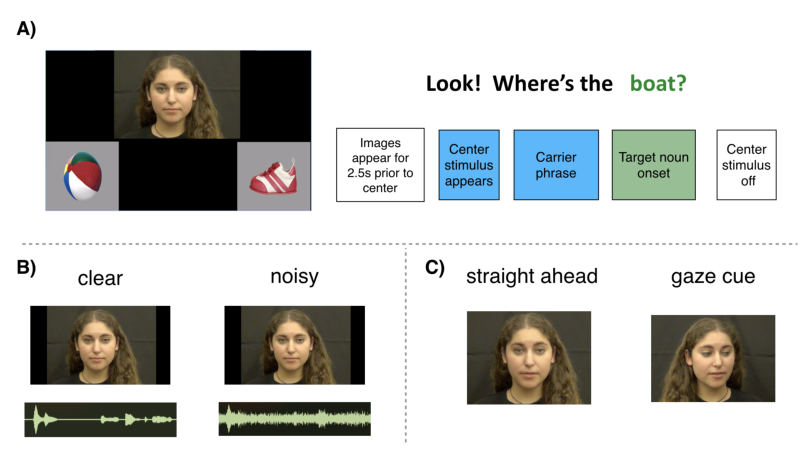
\includegraphics{figs/stimuli-1} 

}

\caption[Stimuli for E1 and E2]{Stimuli for E1 and E2. Panel A shows the layout of the fixation locations for all tasks: the center stimulus, the target, and the distracter. Panel B shows the five center stimulus items: a static geometric shape (Bullseye), a static image of a familiar object (Object), a person speaking (Face), a person signing (ASL), and printed text (Text).}\label{fig:stimuli}
\end{figure*}
\end{CodeChunk}

\subsection{Method}\label{method}

\subsubsection{Participants}\label{participants}

Table 1 contains details about the age distributions of children in all
of four samples.

\subsubsection{Stimuli}\label{stimuli}

\emph{Linguistic stimuli.} All three tasks (Object, Bullseye, and Face)
featured the same female speaker who used natural child-directed speech
and said: ``Look! Where's the (target word)?'' The target words were:
ball, banana, book, cookie, juice, and shoe. For the Face task, a female
native English speaker was video-recorded as she looked straight ahead
and said, ``Look! Where's the (target word)?'' Mean word length was

\emph{Visual stimuli.} The image set consisted of colorful digitized
pictures of objects presented in fixed pairs with no phonological
overlap (ASL task: cat---bird, car---book, bear---doll, ball---shoe;
English tasks: book-shoe, juice-banana, cookie-ball). Side of target
picture was counterbalanced across trials.

\subsubsection{Design and procedure}\label{design-and-procedure}

Children sat on their caregiver's lap and viewed the task on a screen
while their gaze was recorded using a digital camcorder. On each trial,
children saw two images of familiar objects on the screen for two
seconds before the center stimulus appeared (see Fig 1). Then they
processed the target sentence -- which consisted of a carrier phrase, a
target noun, and a question -- followed by two seconds without language
to allow for a response. Participants saw 32 test trials with several
filler trials interspersed to maintain interest.

\emph{Coding.} Participants' gaze patterns were coded (33-ms resolution)
as being fixated on either the center stimulus, one of the images,
shifting between pictures, or away. To assess inter-coder reliability,
25\% of the videos were re-coded. Agreement was scored at the level of
individual frames of video and averaged 98\% on these reliability
assessments.

\subsection{Results and Discussion}\label{results-and-discussion}

\subsubsection{Analysis plan}\label{analysis-plan}

First, we present behavioral analyses of First shift accuracy and
Reaction Time (RT). RT corresponds to the latency to shift away from the
central stimulus to either picture measured from target-noun onset.
Accuracy was the mean proportion of first gaze shifts that landed on the
target picture out of the total number of shifts. We log transformed all
RTs and used the \texttt{lme4} R package (Bates, Maechler, Bolker, \&
Walker, 2013) to fit mixed-effects regression models that included a
random intercept for each participant and item. Since children's age
varied across conditions, we included age in months as a covariate in
all models. All analysis code can be found in the online repository for
this project: \url{https://github.com/kemacdonald/speed-acc/R/analysis}.

Next, we present two exploratory model-based analyses to quantify
differences in eye movements across the four samples. First, we use an
EWMA method to model changes in accuracy as a function of increases in
RT. For each RT, the model generates two values: a ``control statistic''
(CS, which captures the running average accuracy of first shifts) and an
``upper control limit'' (UCL, which captures the pre-defined limit of
when accuracy would be categorized as above chance level). Here, the CS
is an expectation of random shifting to either the target or the
distracter image (nonlanguage-driven shifts), or a Bernoulli process
with probability of success 0.5. As the RTs get longer, we assume that
participants have gathered more information and should become more
accurate, or a Bernoulli process with probability success \textgreater{}
0.5. Using this model, we can quantify and compare: a) the cutoff point
when the CS exceeds the UCL, indicating that participants started to
generate language-driven shifts and b) the proportion of shifts that the
model categorizes as language-driven vs.~nonlanguage-driven.

Finally, we took the shifts that were categorized as language-driven by
the EWMA and fit a hierarchical Bayesian drift-diffusion model (HDDM) to
quantify differences in the speed and accuracy of language-driven eye
movements. We chose to implement a hierarchical Bayesian version of the
DDM using the HDDM Python package (Wiecki, Sofer, \& Frank, 2013) since
we had relatively few trials from child participants and recent
simulation studies have shown that the HDDM approach was better than
other DDM fitting methods for small data sets (Ratcliff \& Childers,
2015). The model assumes that people accumulate noisy evidence in favor
of one alternative with a response generated when the evidence crosses a
pre-defined decision threshold. Here we focus on two parameters of
interest that map onto meaningful psychological variables:
\emph{boundary separation}, which indexes the amount of evidence
gathered before a response (higher values suggest more cautious
responding) and \emph{drift rate}, which indexes the amount of evidence
accumulated per unit time (higher values suggest more efficient
processing).

\begin{CodeChunk}
\begin{figure*}[t]

{\centering 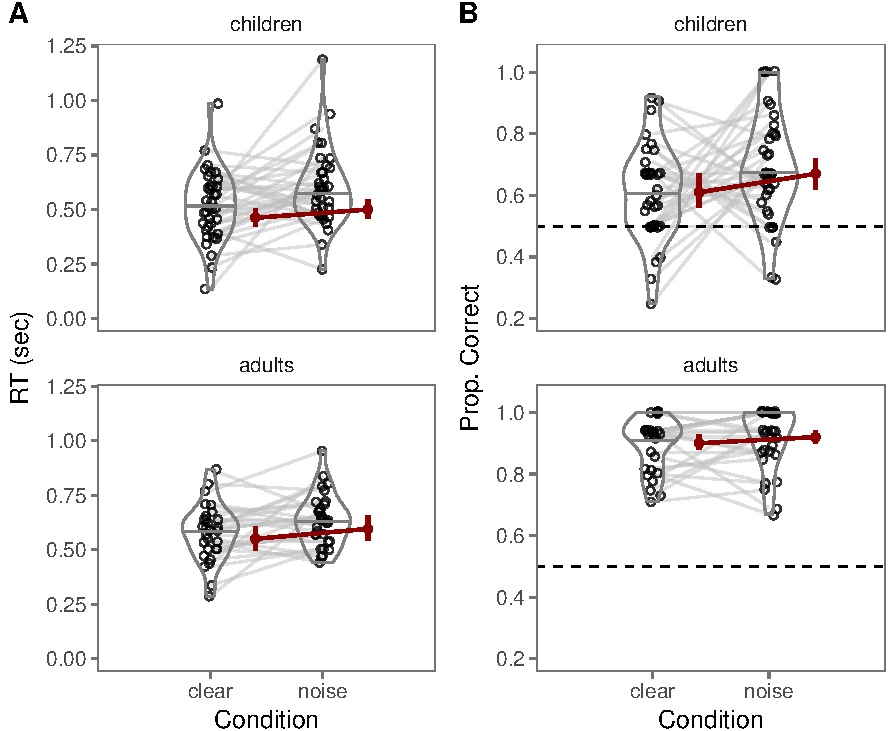
\includegraphics{figs/e1_acc_rt-1} 

}

\caption[First shift accuracy and RTs from E1]{First shift accuracy and RTs from E1. Panel A shows a boxplot representing the distribution of RTs for correct (orange) and incorrect (blue) shifts for each center stimulus type. Panel B shows the distribution of mean first shift accuracy scores for each center stimulus type. The solid lines represent median values, the boundaries of the box show the upper and lower quartiles, and the whiskers show the full range of the data excluding outliers.}\label{fig:e1_acc_rt}
\end{figure*}
\end{CodeChunk}

\subsubsection{Behavioral analyses}\label{behavioral-analyses}

\emph{RT.}

\emph{Accuracy.}

\subsubsection{Model-based analyses}\label{model-based-analyses}

\emph{EWMA.}

\emph{HDDM.}

\section{Experiment 2}\label{experiment-2}

\subsection{Method}\label{method-1}

\subsubsection{Participants}\label{participants-1}

25 Stanford undergraduates participated (5 male, 20 females) for course
credit. All participants were monolingual, native English speakers and
had normal vision.

\subsubsection{Stimuli}\label{stimuli-1}

Audio and visual stimuli were identical to the Face and Bullseye tasks
in E1. We included a new center fixation stimulus type: printed text.
The text was displayed in a white font on a black background and was
programmed such that only a single word appeared on the screen, with
each word appearing for the same duration as the corresponding word in
the spoken language stimuli.

\subsubsection{Design and procedure}\label{design-and-procedure-1}

The design was nearly identical to E1, with the exception of a change to
a within-subjects manipulation where each participant completed all four
tasks (Bullseye, Face, Text, and Text-no-audio). In the Text condition,
spoken language accompanied the printed text. In the Text-no-audio
condition, the spoken language stimulus was removed. Participants saw a
total of 128 trials while their eye movements were tracked using
automated eye-tracking software.

\subsection{Results and Discussion}\label{results-and-discussion-1}

\subsubsection{Behavioral analyses}\label{behavioral-analyses-1}

\emph{RT.}

\emph{Accuracy.}

\subsubsection{Model-based analyses}\label{model-based-analyses-1}

\emph{EWMA.}

\emph{HDDM.}

\section{General Discussion}\label{general-discussion}

Language comprehension can be facilitated by fixating on relevant
features of the nonlinguistic visual world or on the speaker. But how do
we decide where to look? We propose that eye movements during language
processing reflect a sensitivity to the tradeoffs of gathering different
kinds of information. We found that young ASL-learners generated slower
but more accurate shifts away from a language source and produced a
smaller proportion of nonlanguage-driven shifts compared to spoken
language learners. We found the same pattern of behavior within a sample
of English-speaking adults processing displays of printed text compared
to spoken language. These results suggest that as the value of fixating
on a location to gather information about the linguistic signal
increases, eye movements to the \emph{rest} of the visual world become
less useful and occur less often.

Our work here attempts to synthesize results from different populations
and stimuli in a single framework, but it has several limitations that
we hope will pave the way for future work. First, we have not performed
a confirmatory test of the DDM findings: both ASL-learners (E1) and
adults processing language from a person (E2) prioritize accuracy over
speed. So these findings, while interesting, are preliminary. Second, we
do not know what might be driving the population differences in E1. It
could be that ASL-learners' massive experience dealing with competition
for visual attention leads to changes in the deployment of eye movements
during language comprehension. Or, it could be that the in-the-moment
constraints of processing a visual language cause different fixation
behaviors. Finally, we used a very simple visual world, with only three
places to look, and very simple linguistic stimuli, especially for the
adults in E2. Thus it remains an open question how these results might
scale up to more complex language information and visual environments.

This work attempts to integrate top-down, goal-based models of vision
(Hayhoe \& Ballard, 2005) with work on language-driven eye movements
(Allopenna et al., 1998). While we chose to start with two case studies
-- ASL and text processing -- we think the account is more general and
that there are many real world situations where people must negotiate
the tradeoff between gathering more information about language or about
the world: e.g., processing spoken language in noisy environments or at
a distance; or early in language learning when children are acquiring
new words and often rely on nonlinguistic cues to reference such as
pointing or eye gaze. Overall, we hope this work contributes to a
broader account of eye movements during language comprehension that can
explain fixation behaviors across a wider variety of populations,
processing contexts, and during different stages of language learning.

\section{Acknowledgements}\label{acknowledgements}

We are grateful to the families who participated in this research.
Thanks to Tami Alade and Hannah Slater for help with data collection.
This work was supported by an NSF GRFP to KM.

\section{References}\label{references}

\setlength{\parindent}{-0.1in} \setlength{\leftskip}{0.125in} \noindent

\hypertarget{refs}{}
\hypertarget{ref-allopenna1998tracking}{}
Allopenna, P. D., Magnuson, J. S., \& Tanenhaus, M. K. (1998). Tracking
the time course of spoken word recognition using eye movements: Evidence
for continuous mapping models. \emph{Journal of Memory and Language},
\emph{38}(4), 419--439.

\hypertarget{ref-altmann2007real}{}
Altmann, G., \& Kamide, Y. (2007). The real-time mediation of visual
attention by language and world knowledge: Linking anticipatory (and
other) eye movements to linguistic processing. \emph{Journal of Memory
and Language}, \emph{57}(4), 502--518.

\hypertarget{ref-bates2013lme4}{}
Bates, D., Maechler, M., Bolker, B., \& Walker, S. (2013). Lme4: Linear
mixed-effects models using eigen and s4. r package version 1.0-5.

\hypertarget{ref-hayhoe2005eye}{}
Hayhoe, M., \& Ballard, D. (2005). Eye movements in natural behavior.
\emph{Trends in Cognitive Sciences}, \emph{9}(4), 188--194.

\hypertarget{ref-ratcliff2015individual}{}
Ratcliff, R., \& Childers, R. (2015). Individual differences and fitting
methods for the two-choice diffusion model of decision making.
\emph{Decision}, \emph{2}(4), 237--279.

\hypertarget{ref-tanenhaus1995integration}{}
Tanenhaus, M. K., Spivey-Knowlton, M. J., Eberhard, K. M., \& Sedivy, J.
C. (1995). Integration of visual and linguistic information in spoken
language comprehension. \emph{Science}, \emph{268}(5217), 1632.

\hypertarget{ref-vandekerckhove2007fitting}{}
Vandekerckhove, J., \& Tuerlinckx, F. (2007). Fitting the ratcliff
diffusion model to experimental data. \emph{Psychonomic Bulletin \&
Review}, \emph{14}(6), 1011--1026.

\hypertarget{ref-wiecki2013hddm}{}
Wiecki, T. V., Sofer, I., \& Frank, M. J. (2013). HDDM: Hierarchical
bayesian estimation of the drift-diffusion model in python.
\emph{Frontiers in Neuroinformatics}, \emph{7}, 14.

\end{document}
